There are several ways to measure the association between a risk factor and the binary outcome of contracting a disease.
The following sections discuss the four approaches used in this analysis to determine the associated risk of various factors in the context of patients contracting heart disease.
Sections~\ref{subsec:associated-risk-difference} through~\ref{subsec:odds-ratio} refer to table~\ref{tab:contingency} for simplification.

\begin{table}[b]
    \caption{Contingency Matrix}
    \label{tab:contingency}
    \centering
    \begin{tabular}{|r|cc|}
        \hline & {\text{ Diseased }} & {\text{ Healthy }} \\
        \hline {\text{ Exposed }} & $D_E$ & $H_E$ \\
        {\text{ Unexposed }} & $D_U$ & $H_U$ \\ \hline
    \end{tabular}
\end{table}

\subsection{Risk Difference}\label{subsec:associated-risk-difference}

Often considered the simplest approach for measuring associated risk, \emph{risk difference} or \emph{absolute risk difference} (ARD) is the difference in the outcome rates between patients with the risk factor and patients without the risk factor~\citep{Statistical-hypothesis-testing}.
Using the matrix in table~\ref{tab:contingency}, risk difference can be defined mathematically as:
\begin{align*}
 \text{ARD} = \ARD{D_{E}}{H_{E}}{D_{U}}{H_{U}}
\end{align*}
While the risk difference is easy to compute, its interpretation is often misleading and can only explain the associated risk between a single factor and the target.

\subsection{Relative Risk}\label{subsec:relative-risk}
Similar to risk difference, \emph{relative risk} compares the outcome rates between patients with the risk factor and patients without the risk factor.
However, relative risk is computed as a ratio (RR) rather than a difference~\citep{Statistical-hypothesis-testing}.
The risk ratio is defined as:
\begin{align*}
 \text{RR} = \RR{D_{E}}{H_{E}}{D_{U}}{H_{U}}
\end{align*}
Relative risk is a useful statistic because it quantifies the probability of a patient with exposure contracting the disease relative to a patient without exposure.
Risk ratios that are close to $1$ indicate that the risk of contracting the disease for an exposed patient is the same as the risk for an unexposed patient.
In contrast, risk ratios that are far from $1$ indicate that there is an association between the variables.
This allows one to create a confidence interval using the hypothesis test,
\begin{align*}
    H_0&: RR = 1 \\
    H_1&: RR \neq 1
\end{align*}
The risk ratio is considered a valid measure of relative risk for studies in which the sampling is dependent on the exposure of interest such as, randomized controlled trials or cohort and cross-sectional studies~\citep{Relative-Measures-of-Association-for-Binary-Outcomes}.
Like risk difference, relative risk can only explain the associated risk between a single factor and the target.


\subsection{Odds Ratio}
\label{subsec:odds-ratio}
Often confused with risk ratio, \emph{odds ratio} compares the statistical odds of the outcome in the exposed group to that of the outcome of the unexposed group.
It is defined mathematically as:
\begin{align*}
 \text{OR} = \OR{D_{E}}{H_{E}}{D_{U}}{H_{U}}
\end{align*}
Like the risk ratio, odds ratios that are close to $1$ indicate no association between exposure and contracting the disease, and odds ratios that are far from $1$ indicate that there is an association between the variables.
One can also create a confidence interval for the odds ratio using a similar hypothesis test to that of the risk ratio, such that
\begin{align*}
    H_0&: OR = 1 \\
    H_1&: OR \neq 1
\end{align*}
While the odds ratio is typically considered the \enquote{only valid measure of relative association in traditional case-control studies}~\citep{Relative-Measures-of-Association-for-Binary-Outcomes}, it is frequently misinterpreted as the risk ratio.
However, in cases where the risk factor is relatively small ($< 10\%$), the odds ratio approximates the risk ratio:
\begin{align*}
%    \begin{matrix}
%        \Lim{D_E}{0}{D_E + H_E} = H_E \\
%        \Lim{D_U}{0}{D_U + H_U} = H_U
%    \end{matrix} &\implies
    \RR{D_{E}}{H_{E}}{D_{U}}{H_{U}} \approx \OR{D_{E}}{H_{E}}{D_{U}}{H_{U}}
\end{align*}
if $D_E$ and $D_U$ are small.

The odds ratio can be applied in multi-parameter settings when computed in a logistic regression analysis, due to its inherent calculation of the logit (or log-odds) function.
To obtain the odds ratio of a logistic regression model, one simply has to exponentiate the coefficients.


\subsection{Marginal Effects}\label{subsec:marginal-effects}

A \emph{marginal effect} (or incremental effect) is the change in the probability that an outcome occurs as the risk factor changes by one unit.
It is often used in logistic regression analysis and other GLM's to explain the incremental risk associated with each factor~\citep{Marginal-Effects--Quantifying-the-Effect-of-Changes-in-Risk-Factors-in-Logistic-Regression-Models}. 
Unlike the odds ratios, the marginal effects are not a function of the regression coefficients.
Marginal effects are determined by taking the partial derivative of the regression equation with respect to each variable.
They are simpler to interpret than odds ratios and are easier to compare across different studies.
There are many ways to represent the marginal effect for a sample, the most common of which is the \emph{average marginal effect} across all patients in the dataset.

\subsection{The Analysis}\label{subsec:analysis}

\begin{figure*}[btp]
     \centering
     \begin{subfigure}[b]{0.32\textwidth}
         \centering
         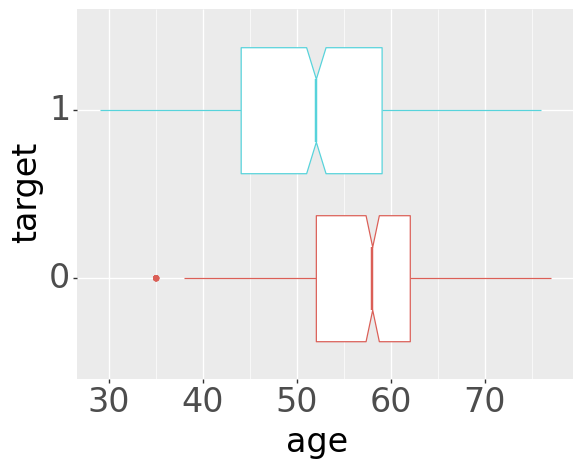
\includegraphics[width=\textwidth]{plots/target-age}
     \end{subfigure}
     \begin{subfigure}[b]{0.32\textwidth}
         \centering
         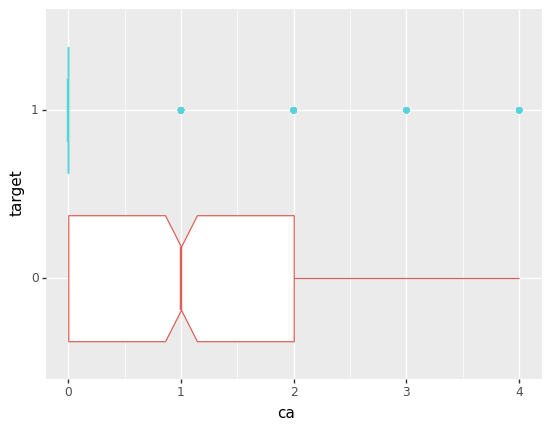
\includegraphics[width=\textwidth]{plots/target-ca}
     \end{subfigure}
     \begin{subfigure}[b]{0.32\textwidth}
         \centering
         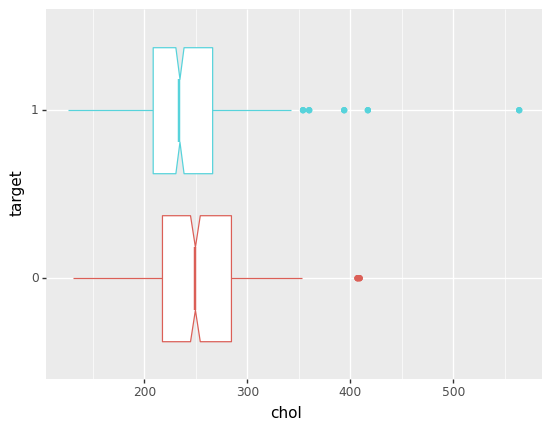
\includegraphics[width=\textwidth]{plots/target-chol}
     \end{subfigure}

     \begin{subfigure}[b]{0.32\textwidth}
         \centering
         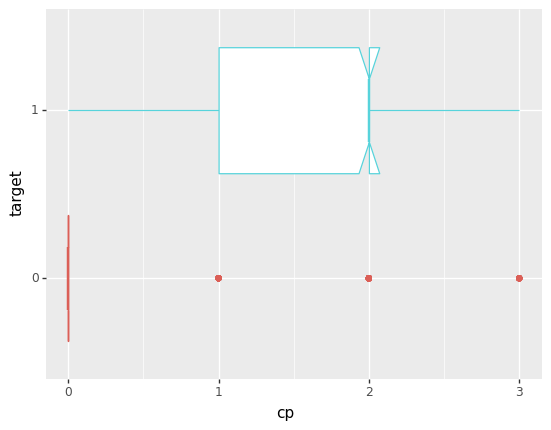
\includegraphics[width=\textwidth]{plots/target-cp}
     \end{subfigure}
     \begin{subfigure}[b]{0.32\textwidth}
         \centering
         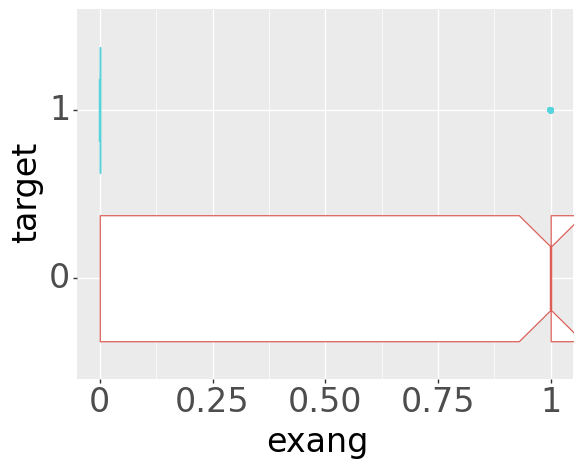
\includegraphics[width=\textwidth]{plots/target-exang}
     \end{subfigure}
     \begin{subfigure}[b]{0.32\textwidth}
         \centering
         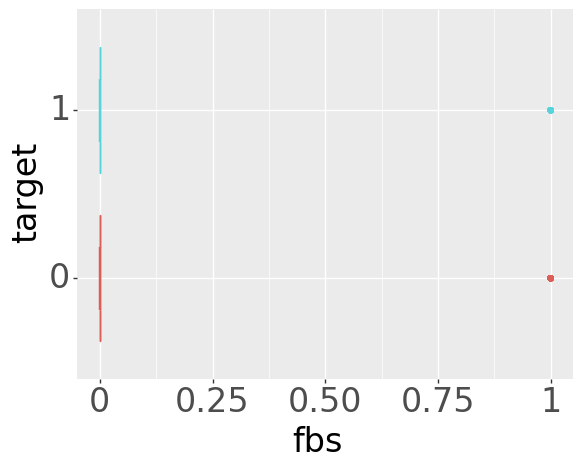
\includegraphics[width=\textwidth]{plots/target-fbs}
     \end{subfigure}

     \begin{subfigure}[b]{0.32\textwidth}
         \centering
         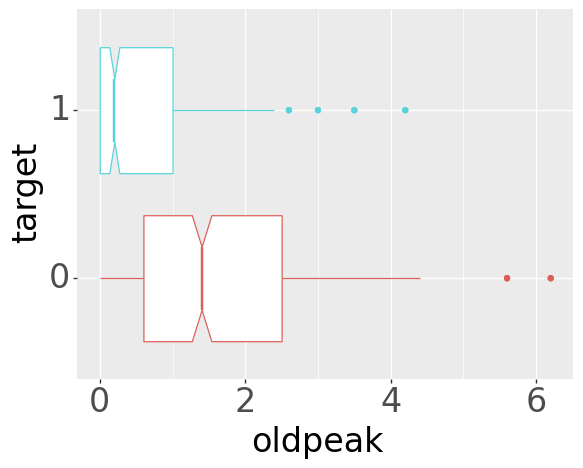
\includegraphics[width=\textwidth]{plots/target-oldpeak}
     \end{subfigure}
     \begin{subfigure}[b]{0.32\textwidth}
         \centering
         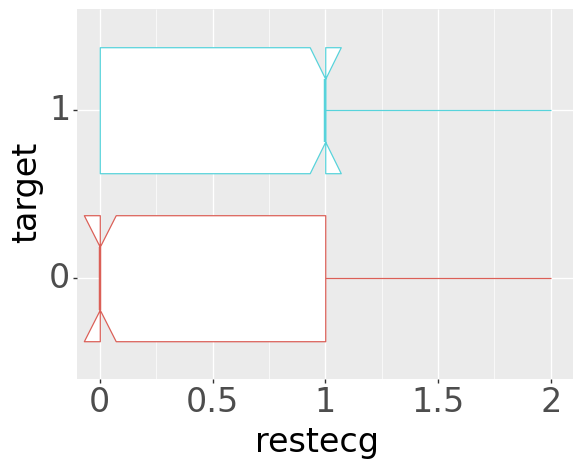
\includegraphics[width=\textwidth]{plots/target-restecg}
     \end{subfigure}
     \begin{subfigure}[b]{0.32\textwidth}
         \centering
         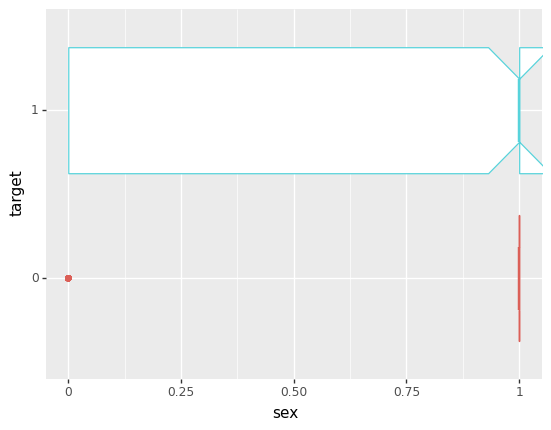
\includegraphics[width=\textwidth]{plots/target-sex}
     \end{subfigure}

     \begin{subfigure}[b]{0.32\textwidth}
         \centering
         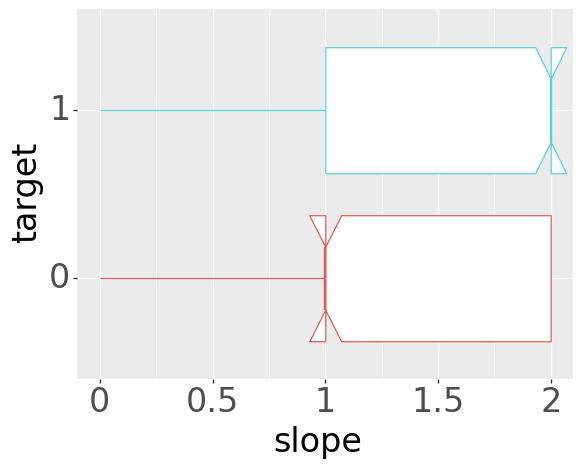
\includegraphics[width=\textwidth]{plots/target-slope}
     \end{subfigure}
     \begin{subfigure}[b]{0.32\textwidth}
         \centering
         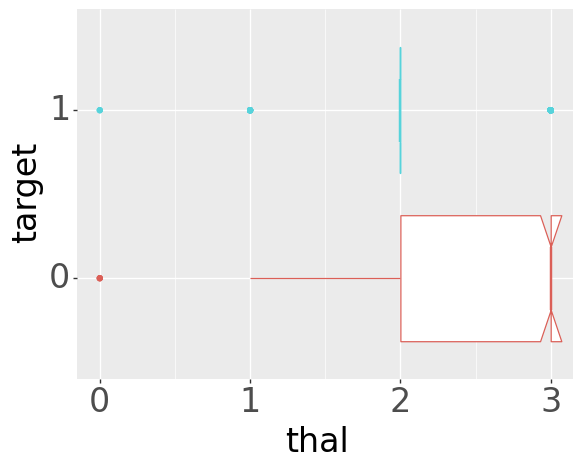
\includegraphics[width=\textwidth]{plots/target-thal}
     \end{subfigure}
     \begin{subfigure}[b]{0.32\textwidth}
         \centering
         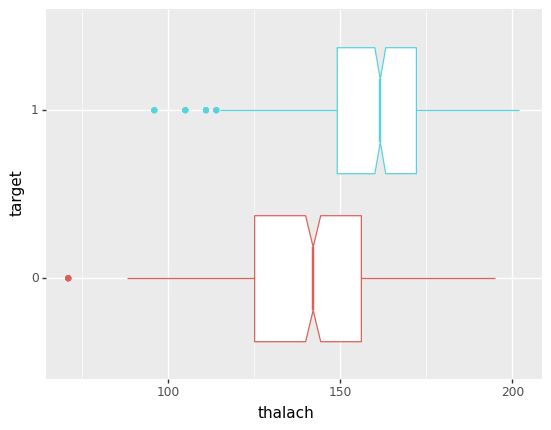
\includegraphics[width=\textwidth]{plots/target-thalach}
     \end{subfigure}

     \begin{subfigure}[b]{0.32\textwidth}
         \centering
         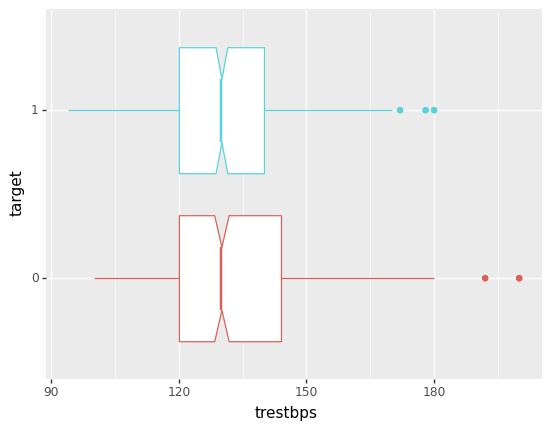
\includegraphics[width=\textwidth]{plots/target-trestbps}
     \end{subfigure}

     \caption[Figure]{Distributions of Feature Variables with Respect to the Target} \label{fig:subdistributions}
\end{figure*}

For this analysis, the \emph{Heart Disease Dataset} was collected from kaggle.com~\citep{Heart-disease-dataset}.
The dataset includes data that was compiled from four databases in 1988 and consists of 1025 rows and 14 columns: 13 predictors and 1 target.
The predictors include 5 continuous variables: age, resting blood pressure, serum cholestoral (in mg/dl), maximum heart rate achieved, and ST depression induced by exercise relative to rest (oldpeak);
and 8 categorical variables: sex, chest pain type, fasting blood sugar $>$ 120 mg/dl (true or false), resting electrocardiographic results, exercise induced angina (yes or no), the slope of the peak exercise ST segment, number of major vessels (0-3) colored by flourosopy, and thal (normal, fixed defect, reversible defect).
Figure~\ref{fig:subdistributions} shows the distributions of predictor variables when compared to the target, a binary indicator for the patient having heart disease and figure~\ref{fig:skim} shows the \inlinecodettt{skimpy} summary of all 14 variables.

\begin{figure*}[tp]
    \centering
    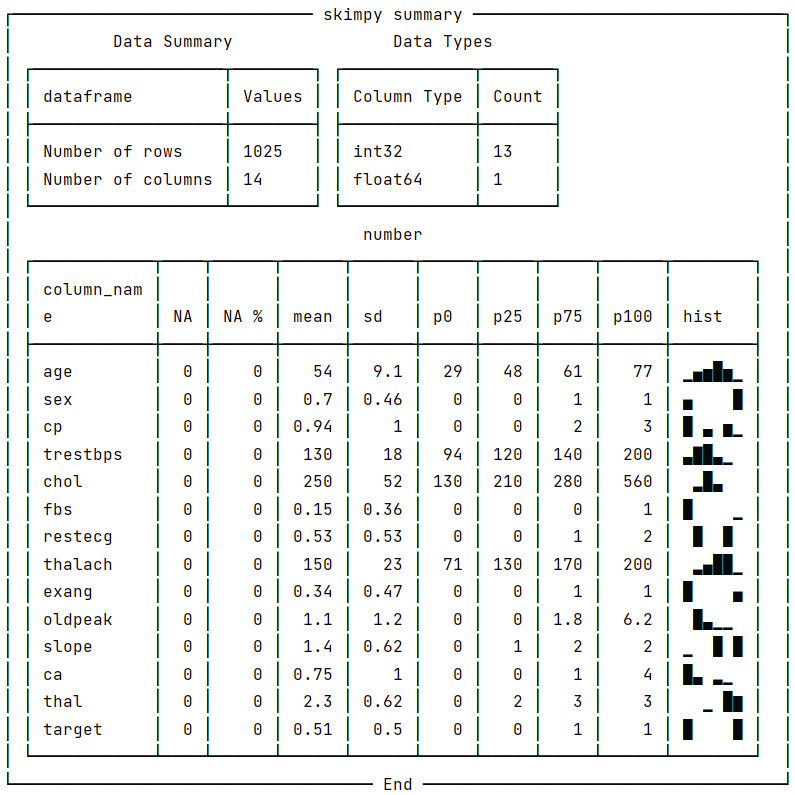
\includegraphics[width=.7\textwidth]{plots/skimpy-summary}
     \caption[Figure]{Summary of Variables} \label{fig:skim}
\end{figure*}

Prior to computing any of the above measures of associated risk, the data was imported into Python (3.9) using \inlinecodettt{pandas} and dummy variables were created for the categorical columns.
Individual risk differences and risk ratios were then computed for each predictor variable.
The dataset was then divided into a $3:2$ train-test split so that a logistic regression model can be fit.
Two models were fit using the training set to the objective function,
\begin{align*}
    \logit{Y} = \vec{\beta}\matrx{X}
\end{align*}
via \inlinecodettt{statsmodels}.
One was computed with the odds ratio, and the other with marginal effects.
The models were then tested with the remainder of the data and scored using \inlinecodettt{sklearn}.

%%%%%%%%%%%%%%%%%

\begin{table*}[!bp]
    \caption{Risk Difference and Risk Ratio of Binary Variables} 
    \label{tab:risk}
    \colorbox{gray!20}{
    \resizebox{\textwidth}{!}{
        \begin{tabular}{lrrr}
        \toprule
        {} & Risk Difference & Risk Ratio & RR 95\% Confidence Interval \\
        \midrule
        age                               &         -0.2892 &     0.5671 &          (0.5008, 0.6423)^* \\
        sex                               &         -0.3036 &     0.5809 &          (0.5204, 0.6484)^* \\
        resting blood pressure $>$ 130      &         -0.0888 &      0.839 &          (0.7411, 0.9499)^* \\
        serum cholestoral $>$ 250 ml/dl     &         -0.1512 &     0.7374 &          (0.6473, 0.8401)^* \\
        fasting blood sugar $>$ 120 mg/dl   &         -0.0577 &     0.8893 &           (0.7415, 1.0666) \\
        maximum heart rate achieved $>$ 150 &          0.4067 &      2.364 &          (2.0403, 2.7391)^* \\
        exercise induced angina           &         -0.4633 &     0.3076 &          (0.2483, 0.3809)^* \\
        oldpeak                           &         -0.3773 &      0.435 &          (0.3708, 0.5103)^* \\
        chest pain = 1                    &          0.3455 &     1.7563 &          (1.5815, 1.9503)^* \\
        chest pain = 2                    &          0.3568 &     1.8613 &          (1.6732, 2.0704)^* \\
        chest pain = 3                    &          0.1613 &     1.3219 &          (1.1134, 1.5694)^* \\
        resting electrocardiograph = 1    &          0.1785 &     1.4212 &          (1.2566, 1.6073)^* \\
        resting electrocardiograph = 2    &         -0.3178 &     0.3862 &           (0.1401, 1.0646) \\
        slope = 1                         &         -0.3499 &     0.4837 &          (0.4203, 0.5566)^* \\
        slope = 2                         &          0.3904 &      2.167 &          (1.9032, 2.4674)^* \\
        major vessels colored = 1         &         -0.2837 &     0.5073 &          (0.4105, 0.6268)^* \\
        major vessels colored = 2         &         -0.4101 &     0.2765 &          (0.1859, 0.4112)^* \\
        major vessels colored = 3         &         -0.4104 &     0.2412 &          (0.1308, 0.4448)^* \\
        major vessels colored = 4         &          0.3259 &     1.6422 &           (1.324, 2.0369)^* \\
        thal = 1                          &         -0.1974 &     0.6244 &          (0.4375, 0.8911)^* \\
        thal = 2                          &          0.5203 &     3.1955 &          (2.7033, 3.7772)^* \\
        thal = 3                          &         -0.4894 &     0.3096 &          (0.2562, 0.3742)^* \\
        \bottomrule
        \end{tabular}
    }}
\end{table*}

\begin{table*}[!tp]
\small
\colorbox{gray!20}{
    \resizebox{\textwidth}{!}{
        \begin{tabular}{c}
        \toprule
        \begin{tabular*}{\textwidth}{lr @{\extracolsep{\fill}} lr}
        \textbf{Dep. Variable:}   &      target      & \textbf{  No. Observations:  } &      615    \\
        \textbf{Model:}           &      Logit       & \textbf{  Df Residuals:      } &      593    \\
        \textbf{Method:}          &       MLE        & \textbf{  Df Model:          } &       21    \\
        \textbf{Date:}            & Mon, 28 Nov 2022 & \textbf{  Pseudo R-squ.:     } &   0.5868    \\
        \textbf{Time:}            &     20:02:19     & \textbf{  Log-Likelihood:    } &   -175.99   \\
        \textbf{converged:}       &       True       & \textbf{  LL-Null:           } &   -425.93   \\
        \textbf{Covariance Type:} &    nonrobust     & \textbf{  LLR p-value:       } & 1.574e-92   \\
        \end{tabular*}    \\
        \bottomrule
        
        \begin{tabular*}{\textwidth}{l  @{\extracolsep{\fill}} rrrrrr}
                            & \textbf{coef} & \textbf{std err} & \textbf{z} & \textbf{P$> |$z$|$} & \textbf{[0.025} & \textbf{0.975]}  \\
        \midrule
        
        \textbf{age}                               &       0.0376  &        0.018     &     2.080  &         0.038        &        0.002    &        0.073     \\
        \textbf{sex}                               &      -2.2499  &        0.433     &    -5.195  &         0.000        &       -3.099    &       -1.401     \\
        \textbf{resting blood pressure}            &      -0.0244  &        0.009     &    -2.857  &         0.004        &       -0.041    &       -0.008     \\
        \textbf{serum cholesterol}                 &      -0.0145  &        0.004     &    -3.853  &         0.000        &       -0.022    &       -0.007     \\
        \textbf{fasting blood sugar $>$ 120 mg/dl} &       0.2915  &        0.441     &     0.661  &         0.509        &       -0.573    &        1.156     \\
        \textbf{maximum heart rate achieved}       &       0.0242  &        0.008     &     2.953  &         0.003        &        0.008    &        0.040     \\
        \textbf{exercise induced angina}           &      -0.4887  &        0.321     &    -1.523  &         0.128        &       -1.118    &        0.140     \\
        \textbf{oldpeak}                           &      -0.5662  &        0.177     &    -3.206  &         0.001        &       -0.912    &       -0.220     \\
        \textbf{chest pain = 1}                    &       0.9770  &        0.421     &     2.320  &         0.020        &        0.152    &        1.802     \\
        \textbf{chest pain = 2}                    &       1.8772  &        0.380     &     4.942  &         0.000        &        1.133    &        2.622     \\
        \textbf{chest pain = 3}                    &       2.4143  &        0.497     &     4.854  &         0.000        &        1.439    &        3.389     \\
        \textbf{resting electrocardiograph = 1}    &       0.1241  &        0.286     &     0.434  &         0.664        &       -0.436    &        0.685     \\
        \textbf{resting electrocardiograph = 2}    &      -0.9711  &        3.222     &    -0.301  &         0.763        &       -7.286    &        5.344     \\
        \textbf{slope = 1}                         &      -0.6824  &        0.610     &    -1.118  &         0.264        &       -1.879    &        0.514     \\
        \textbf{slope = 2}                         &       0.8047  &        0.657     &     1.224  &         0.221        &       -0.484    &        2.093     \\
        \textbf{major vessels colored = 1}         &      -2.4127  &        0.394     &    -6.126  &         0.000        &       -3.185    &       -1.641     \\
        \textbf{major vessels colored = 2}         &      -3.3407  &        0.553     &    -6.041  &         0.000        &       -4.425    &       -2.257     \\
        \textbf{major vessels colored = 3}         &      -2.3139  &        0.697     &    -3.319  &         0.001        &       -3.680    &       -0.947     \\
        \textbf{major vessels colored = 4}         &       1.2003  &        1.213     &     0.990  &         0.322        &       -1.177    &        3.577     \\
        \textbf{thalassemia = 1}                   &       4.1461  &        1.976     &     2.098  &         0.036        &        0.273    &        8.019     \\
        \textbf{thalassemia = 2}                   &       3.9308  &        1.967     &     1.999  &         0.046        &        0.076    &        7.785     \\
        \textbf{thalassemia = 3}                   &       2.6183  &        1.976     &     1.325  &         0.185        &       -1.255    &        6.492     \\

        \end{tabular*}  \\
        \bottomrule
        \end{tabular}
    }
}

\caption{Logistic Regression Results}\label{tab:logit-regression}
\end{table*}

Table \ref{tab:risk} shows the risk difference and the relative risk of feature variables when compared against the target.
The variable with the highest risk difference is \emph{thal = 2}, with a difference of $0.5203$; meaning, on average, in a sample of $100$ patients $52$ more patients who have Thalassemia (a blood disease characterized by low hemoglobin production) as a fixed defect will contract heart disease than patients without Thalassemia.
The variable with the lowest risk difference is is \emph{thal = 3} with a difference of $-0.4894$; meaning, on average, in a sample of $100$ patients $49$ fewer patients who have Thalassemia as a reversible defect will contract heart disease than patients without Thalassemia. 
Comparing the risk difference to the risk ratio, variables with risk differences less than zero have risk ratios less than 1 and variables with risk differences greater than zero have risk ratios greater than 1. 
Of the 22 risk ratios, only 2 variables have confidence intervals that contain 1, and thus accept the null-hypothesis. 
The variable with the highest statistically significant risk ratio is \emph{thal = 2}, with a risk ratio of $3.1955$; meaning, patients who have Thalassemia as a fixed defect are $3.1955$ times more likely to contract heart disease than patients without Thalassemia.
The variable with the lowest statistically significant risk ratio is \emph{major vessels colored = 3}, with a risk ratio of $0.2412$; meaning, patients who had 3 major blood vessels colored in a flourosopy are $0.2412$ times less likely to contract heart disease than patients who had no major blood vessels colored in a flourosopy.


To compute the odds ratios and the marginal effects, two logistic regression models were fit; one using the maximum likelihood method and the other using the average marginal effects.
Table~\ref{tab:logit-regression} shows the regression results for the maximum likelihood model.
The log-likelihood of the model is $-175.99$, which is significantly larger than the log-likelihood of the null-model, $-425.93$, given the log-likelihood ratio test p-value of $1.574\mathrm{e-}92$.

Table \ref{tab:odds} shows the odds ratios of the regression, which were obtained by exponentiating the coefficients in table \ref{tab:logit-regression}.
Of the 22 odds ratios, 8 variables have confidence intervals that contain 1, and thus accept the null-hypothesis.
The variable with the highest statistically significant odds\def\arraystretch{0.5}
\begin{wraptable}{r}{.55\textwidth}
% \begin{table^^*}[h]
% \small
\centering\caption{Odds Ratios}\label{tab:odds}
\colorbox{gray!20}{
\resizebox{.5\textwidth}{!}{
    \begin{tabular}{lrr}
    \toprule
    {} &  Odds Ratio & OR 95\% Confidence Interval \\
    \midrule
    age       &      1.0383 &          (1.0022, 1.0758)^* \\
    sex       &      0.1054 &          (0.0451, 0.2463)^* \\
    trestbps  &      0.9759 &          (0.9597, 0.9924)^* \\
    chol      &      0.9856 &          (0.9784, 0.9929)^* \\
    fbs       &      1.3384 &           (0.5639, 3.1764) \\
    thalach   &      1.0245 &          (1.0082, 1.0411)^* \\
    exang     &      0.6134 &           (0.3271, 1.1505) \\
    oldpeak   &      0.5677 &          (0.4016, 0.8025)^* \\
    cp\_1      &      2.6565 &          (1.1638, 6.0638)^* \\
    cp\_2      &      6.5352 &          (3.104, 13.7594)^* \\
    cp\_3      &     11.1815 &         (4.2184, 29.6385)^* \\
    restecg\_1 &      1.1322 &           (0.6464, 1.9829) \\
    restecg\_2 &      0.3787 &         (0.0007, 209.2937) \\
    slope\_1   &      0.5054 &           (0.1528, 1.6717) \\
    slope\_2   &      2.2360 &           (0.6163, 8.1119) \\
    ca\_1      &      0.0896 &          (0.0414, 0.1938)^* \\
    ca\_2      &      0.0354 &           (0.012, 0.1047)^* \\
    ca\_3      &      0.0989 &          (0.0252, 0.3878)^* \\
    ca\_4      &      3.3210 &          (0.3082, 35.7816) \\
    thal\_1    &     63.1862 &       (1.3143, 3037.8507)^* \\
    thal\_2    &     50.9487 &       (1.0792, 2405.3763)^* \\
    thal\_3    &     13.7129 &          (0.285, 659.8043) \\
    \bottomrule
    \end{tabular}
}
}
% \end{table^^*}
\end{wraptable}
ratio is \emph{thal = 1}, with an odds ratio of $63.1862$; meaning, the odds of contacting heart disease are $63.1862$ times higher for patients with normal Thalassemia than patients without Thalassemia.
The variable with the lowest statistically significant odds ratio is \emph{major vessels colored = 2}, with an odds ratio of $0.0354$; meaning, the odds of contacting heart disease are $0.0354$ times lower for patients who had two major blood vessels colored by a fluoroscopy than patients who had no major blood vessels colored by a fluoroscopy.

Table \ref{tab:marginal} shows the marginal effects of the regression output. Of the 22 marginal effects, 8 variables have p-values greater than $5\%$, and thus accept the null-hypothesis. 
It's important to note that these are the same variables that have statistically insignificant odds ratios.
The variable with the highest statistically significant marginal effect is \emph{thal = 1}, with an average marginal effect of $0.3661$; meaning that the average change in probability is $0.3661$ when a patient has normal Thalassemia. 
The variable with the lowest statistically significant marginal effect is \emph{major vessels colored = 2}, with an average marginal effect of $-0.2949$; meaning that the average change in probability is $-0.2949$ when a patient who has two major blood vessels colored by a fluoroscopy.



\def\arraystretch{1}
\begin{table*}[!tp]

\small
\colorbox{gray!20}{
    \resizebox{\textwidth}{!}{
    \begin{tabular}{c}
        \toprule
    \begin{tabular*}{\textwidth}{lc}
        \textbf{Dep. Variable:} &     target      \\
        \textbf{Method:}        &      dydx       \\
        \textbf{At:}            &    overall      \\
    \end{tabular*} \\
        \bottomrule

\begin{tabular*}{\textwidth}{l @{\extracolsep{\fill}} rrrrrr}
     \textbf{}      & \textbf{dy/dx} & \textbf{std err} & \textbf{z} & \textbf{P$> |$z$|$} & \textbf{[0.025} & \textbf{0.975]}  \\
\midrule

\textbf{age}        &       0.0033   &        0.002     &     2.109  &         0.035        &        0.000    &        0.006     \\
\textbf{sex}        &      -0.1986   &        0.035     &    -5.658  &         0.000        &       -0.267    &       -0.130     \\
\textbf{trestbps}   &      -0.0022   &        0.001     &    -2.915  &         0.004        &       -0.004    &       -0.001     \\
\textbf{chol}       &      -0.0013   &        0.000     &    -4.070  &         0.000        &       -0.002    &       -0.001     \\
\textbf{fbs}        &       0.0257   &        0.039     &     0.662  &         0.508        &       -0.050    &        0.102     \\
\textbf{thalach}    &       0.0021   &        0.001     &     3.038  &         0.002        &        0.001    &        0.004     \\
\textbf{exang}      &      -0.0431   &        0.028     &    -1.533  &         0.125        &       -0.098    &        0.012     \\
\textbf{oldpeak}    &      -0.0500   &        0.015     &    -3.324  &         0.001        &       -0.079    &       -0.021     \\
\textbf{cp\_1}      &       0.0863   &        0.036     &     2.378  &         0.017        &        0.015    &        0.157     \\
\textbf{cp\_2}      &       0.1657   &        0.031     &     5.338  &         0.000        &        0.105    &        0.227     \\
\textbf{cp\_3}      &       0.2132   &        0.041     &     5.210  &         0.000        &        0.133    &        0.293     \\
\textbf{restecg\_1} &       0.0110   &        0.025     &     0.434  &         0.664        &       -0.039    &        0.060     \\
\textbf{restecg\_2} &      -0.0857   &        0.284     &    -0.301  &         0.763        &       -0.643    &        0.472     \\
\textbf{slope\_1}   &      -0.0602   &        0.054     &    -1.122  &         0.262        &       -0.166    &        0.045     \\
\textbf{slope\_2}   &       0.0710   &        0.058     &     1.229  &         0.219        &       -0.042    &        0.184     \\
\textbf{ca\_1}      &      -0.2130   &        0.030     &    -7.037  &         0.000        &       -0.272    &       -0.154     \\
\textbf{ca\_2}      &      -0.2949   &        0.043     &    -6.804  &         0.000        &       -0.380    &       -0.210     \\
\textbf{ca\_3}      &      -0.2043   &        0.059     &    -3.447  &         0.001        &       -0.320    &       -0.088     \\
\textbf{ca\_4}      &       0.1060   &        0.107     &     0.991  &         0.322        &       -0.104    &        0.316     \\
\textbf{thal\_1}    &       0.3661   &        0.172     &     2.124  &         0.034        &        0.028    &        0.704     \\
\textbf{thal\_2}    &       0.3470   &        0.172     &     2.022  &         0.043        &        0.011    &        0.683     \\
\textbf{thal\_3}    &       0.2312   &        0.174     &     1.331  &         0.183        &       -0.109    &        0.572     \\

\end{tabular*} \\
    \bottomrule
\end{tabular}
}
}

\caption{Marginal Effects}\label{tab:marginal}
\end{table*}
